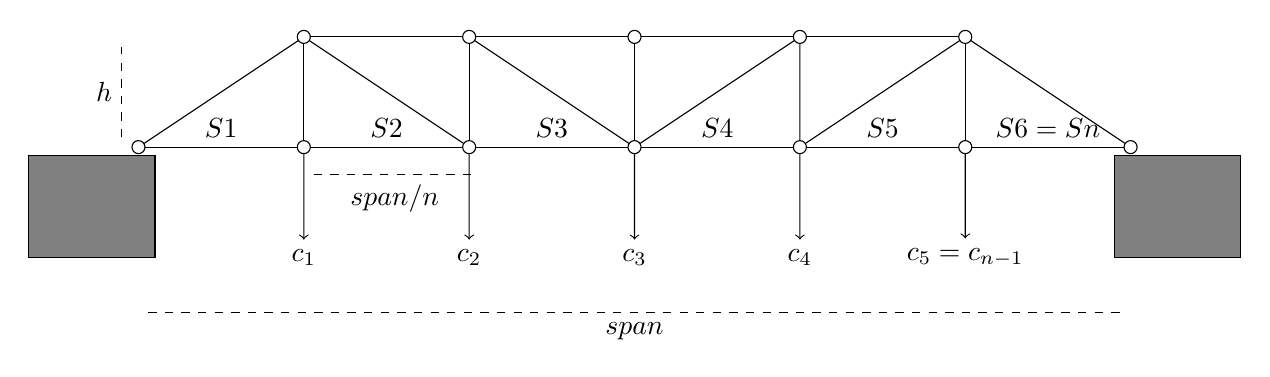
\begin{tikzpicture}[scale = 0.7]

    \tikzset{nodestyle/.style={draw,shape=circle,scale=0.5}}
    \node[nodestyle] (p1) at ( 0, 0) {}; 
    \node[nodestyle] (p2) at ( 3, 0) {};
    \node[nodestyle] (p3) at ( 6, 0) {};
    \node[nodestyle] (p4) at ( 9, 0) {};
    \node[nodestyle] (p5) at ( 12, 0) {};
    \node[nodestyle] (p6) at ( 15, 0) {};
    \node[nodestyle] (p7) at ( 18, 0) {};

    \node[nodestyle] (p8) at ( 3, 2) {};
    \node[nodestyle] (p9) at ( 6, 2) {};
    \node[nodestyle] (p10) at ( 9, 2) {};
    \node[nodestyle] (p11) at ( 12, 2) {};
    \node[nodestyle] (p12) at ( 15, 2) {};

    \begin{scope}[every path/.style={-}]
        \draw (p1) -- (p2) node[midway,above] {$S1$};
        \draw (p2) -- (p3) node[midway,above] {$S2$}; 
        \draw (p3) -- (p4) node[midway,above] {$S3$};
        \draw (p4) -- (p5) node[midway,above] {$S4$};
        \draw (p5) -- (p6) node[midway,above] {$S5$};
        \draw (p6) -- (p7) node[midway,above] {$S6= Sn$};

        \draw (p8) -- (p9);
        \draw (p9) -- (p10);
        \draw (p10) -- (p11);
        \draw (p11) -- (p12);

        \draw (p1) -- (p8);
        \draw (p12) -- (p7);

        \draw (p2) -- (p8);
        \draw (p3) -- (p9);
        \draw (p4) -- (p10);
        \draw (p5) -- (p11);
        \draw (p6) -- (p12);

        \draw (p8) -- (p3);
        \draw (p9) -- (p4);
        \draw (p4) -- (p11);
        \draw (p5) -- (p12);
    \end{scope}  

        \draw[fill=gray] (0.3,-0.15) rectangle (-2,-2);
        \draw[fill=gray] (17.7,-0.15) rectangle (20,-2);

        % Nodos artificiales.
        \node (a1) at ( 0, -3) {};
        \node (a2) at ( 18, -3) {};
        \node (a3) at ( -0.3, 0) {};
        \node (a4) at ( -0.3, 2) {};
        \node (a5) at ( 3, -0.5) {};
        \node (a6) at ( 6.3, -0.5) {};
		\node (c1) at ( 3, -2) {$c_1$};
    \node (c2) at ( 6, -2) {$c_2$};
    \node (c3) at ( 9, -2) {$c_3$};
    \node (c4) at ( 12, -2) {$c_4$};
    \node (c5) at ( 15, -2) {$c_5  = c_{n-1}$};
    \draw[->] (p2) -- (c1);
  	\draw[->] (p3) -- (c2);
   	\draw[->] (p4) -- (c3);
    \draw[->] (p5) -- (c4);
    \draw[->] (p6) -- (c5);        
        
        
        \begin{scope}[every path/.style={-}]
            \draw[dashed] (a1) -- (a2) node[below,midway]{$span$} ;
            \draw[dashed] (a3) -- (a4) node[left,midway]{$h$};
            \draw[dashed] (a5) -- (a6) node[below,midway]{$span/n$};
        \end{scope}
        
\end{tikzpicture}